\section{Tổ chức lưu trữ miền tri thức} 
	Tổ chức lưu trữ miền tri thức trong hệ quản trị cơ sở dữ liệu \texttt{(CSDL) MS SQL Server} với các bảng sau:

\begin{itemize}
	\item Bảng \textbf{\texttt{Vertexs}}: mỗi dòng định danh đỉnh của đồ thị ($a$, $b$, $c$, $\dots$) với \texttt{id} là dãy số duy nhất cho từng đỉnh, \texttt{name} là tên đỉnh thường được đặt theo ký hiệu toán học và \texttt{degree} là thuộc tính bậc của đỉnh (${deg_a}$ = 2, ${deg_b}$ = 1 , $\dots$), trong đó một số trường hợp đặc biệt số bậc của đỉnh như ${deg_b}$ = 1, cho biết $b$ là đỉnh treo hay nếu ${deg_b}$ = 0 thì  $b$ là đỉnh cô lập.
	
	\begin{tabular}{|c|l|}
		\hline
		\multicolumn{2}{|c|}{\textbf{Vertexs}} \\
		\hline
		\textbf{PK} & \texttt{\textbf{id int NOT NULL}} \\
		\hline
		& \texttt{name char(50) NOT NULL} \\
		\hline
		& \texttt{degree int NOT NULL} \\
		\hline
	\end{tabular}
	
	\item Bảng \textbf{\texttt{Edges}}: mỗi dòng chứa thông tin của 1 cạnh trong đồ thị bao gồm 2 \texttt{id} của đỉnh và độ dài của cạnh.
	
	\begin{tabular}{|c|l|}
		\hline
		\multicolumn{2}{|c|}{\textbf{Edges}} \\
		\hline
		\textbf{FK} & \texttt{\textbf{ver\_1 char(50) NOT NULL}} \\
		\hline
		\textbf{FK} & \texttt{\textbf{ver\_2 char(50) NOT NULL}} \\
		\hline
		& \texttt{dist int NOT NULL} \\
		\hline
	\end{tabular}
	
\end{itemize}		
Miền tri thức trên cho phép giải các bài toán liên quan tới phân loại đồ thị, tính đường đi và chu trình đường đi trong đồ thị.

Ví dụ minh họa chi tiết miền tri thức đồ thị hàm số bằng cấu trúc bảng dữ liệu lưu trữ tri thức của đồ thị gồm 5 cạnh a,b,c,d và e với độ dài các cạnh tương ứng như bên dưới

\begin{figure}[h]
	\centering
	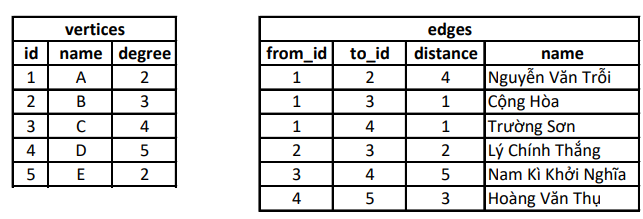
\includegraphics[width= 0.9\linewidth]{tables.PNG}
	\caption{Minh họa miền tri thức định dạng bảng trong CSDL}
	\label{fig-3: dinh dang mien-tri-thuc}
\end{figure}

Trong bài tập, nhóm em sử dụng kiến thức về lập trình hướng đối tượng để xử lý tự động các file được lưu trữ dưới dạng bảng trong MS SQL Server. Lớp đối tượng DOTHI được định nghĩa như sau:

\begin{figure}[h]
	\centering
	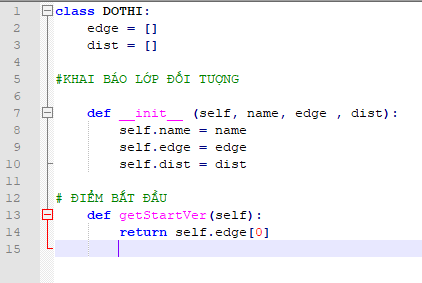
\includegraphics[width=0.8 \linewidth]{DOTHI.PNG}
	\caption{Lớp đối tượng DOTHI}
	\label{fig-3:lop doi tuong do thi}
\end{figure}


Trong đó các biến được định nghĩa như sau:
\begin{itemize}
	\item \texttt{edge} cạnh được tạo thành từ các cặp đỉnh của đồ thị, \texttt{edge} có định dạng: [$a$, $b$].
	\item \texttt{dist} là độ dài của cạnh
	\item \texttt{startPoint} là là điểm đầu tiên trong \texttt{edge}: \texttt{edge}[0]
\end{itemize}